\chapter{Programmazione Ibrida}
Al giorno d'oggi, i sistemi di calcolo ad alte prestazioni moderni non sono più solamente a memoria condivisa o solamente a memoria distribuita, in realtà ci troviamo spesso a dover gestire architetture a memoria distribuita in cui i vari nodi all'interno adottano un modello a memoria condivisa. La scelta più logica è dunque \textbf{combinare il threading a livello del singolo nodo e MPI tra i vari nodi}. 
\section{Perché MPI + OpenMP?}
Sebbene l'approccio ibrido sembri la soluzione ovvia per le moderne architetture di calcolo, la realtà introduce diverse complicazioni tecniche. Di seguito un confronto tra le aspettative teoriche e le sfide pratiche da affrontare:

\subsection*{1. L'adattamento alla struttura gerarchica}
\begin{itemize}
    \item \textbf{Aspettativa:} Il codice si adatta naturalmente ai nodi moderni (threading per i multicore all'interno, MPI per la comunicazione tra i nodi).
    \item \textbf{Realtà:} OpenMP introduce nuove complessità che devono essere gestite accuratamente dal programmatore:
    \begin{itemize}
        \item \textit{Architettura NUMA (Non-Uniform Memory Access):} I core accedono più velocemente alla porzione di memoria RAM fisicamente vicina al loro socket. Se i thread non sono gestiti bene, subiscono ritardi accedendo a memoria "lontana".
        \item \textit{Affinità (Pinning):} È fondamentale assicurarsi che un thread rimanga in esecuzione sempre sullo stesso core per sfruttare la memoria Cache.
        \item \textit{Overhead:} Creare, gestire e distruggere i thread ha un costo computazionale  (il cosiddetto "vaso di Pandora") non indifferente.
    \end{itemize}
\end{itemize}

\subsection*{2. La riduzione del volume di comunicazione}
\begin{itemize}
    \item \textbf{Aspettativa:} Riducendo i processi MPI (es. uno solo per nodo), si riduce il volume dei messaggi inviati sulla rete.
    \item \textbf{Realtà:} La comunicazione MPI può essere altamente ottimizzata anche in programmi non ibridi (ad esempio raggruppando i messaggi). Pertanto, il volume di traffico tra i nodi potrebbe rimanere invariato rispetto a un codice puro MPI ben scritto.
\end{itemize}

\subsection*{3. L'efficienza e la leggerezza di OpenMP}
\begin{itemize}
    \item \textbf{Aspettativa:} I thread OpenMP sono più leggeri dei processi MPI, risultando più efficienti a livello di singolo nodo.
    \item \textbf{Realtà:} Dipende interamente dal codice. Spesso le librerie MPI moderne sono estremamente ottimizzate per la comunicazione intra-nodo (sfruttando la memoria condivisa dietro le quinte). Di conseguenza, una latenza MPI locale può risultare persino inferiore al tempo richiesto per sincronizzare i thread con una barriera OpenMP su un intero nodo.
\end{itemize}


\vspace{0.5cm}
\noindent
\begin{quote}
    \textbf{Riepilogo:} Non esiste una risposta definitiva o una formula magica. Ottenere vantaggi prestazionali reali con la programmazione ibrida è complesso e richiede un'attenta calibrazione sull'hardware.
\end{quote}

\section{Interoperabilità dei thread in MPI}

Per scrivere un programma ibrido, è necessario informare l'ambiente MPI che si intende utilizzare il multithreading. Per farlo, si sostituisce la classica funzione di inizializzazione con \texttt{MPI\_Init\_thread()}.

\subsection*{La funzione MPI\_Init\_thread}
\begin{verbatim}
int MPI_Init_thread(int *argc, char ***argv,
                    int required,     // input
                    int *provided);   // output
\end{verbatim}
Il parametro \texttt{provided} restituito dalla funzione può essere inferiore o superiore al valore \texttt{required} richiesto dall'applicazione. È responsabilità del programmatore gestire eventuali discrepanze.

\subsection*{Livelli di supporto (in ordine crescente)}
I valori passati a \texttt{required} possono essere:
\begin{itemize}
    \item \textbf{\texttt{MPI\_THREAD\_SINGLE}:} Esegue solo un thread (equivalente all'uso standard di \texttt{MPI\_Init()}).
    \item \textbf{\texttt{MPI\_THREAD\_FUNNELED}:} Il programma usa i thread, ma \textit{solo il master thread} effettuerà le chiamate MPI. (Questo è il minimo richiesto per qualsiasi threading con MPI).
    \item \textbf{\texttt{MPI\_THREAD\_SERIALIZED}:} Diversi thread possono effettuare chiamate MPI, ma \textit{solo uno per volta} (la mutua esclusione deve essere garantita dal programmatore).
    \item \textbf{\texttt{MPI\_THREAD\_MULTIPLE}:} Diversi thread possono effettuare chiamate MPI contemporaneamente e senza alcuna restrizione.
\end{itemize}

\subsection{Il pattern base: OpenMP dentro, MPI fuori}
Il pattern più comune e sicuro nella programmazione ibrida si basa su una netta separazione delle responsabilità: MPI si occupa esclusivamente della comunicazione tra i processi, mentre OpenMP gestisce la parallelizzazione del calcolo a livello locale. \textbf{Le due fasi non si sovrappongono mai.}
\begin{figure}[H]
    \centering
    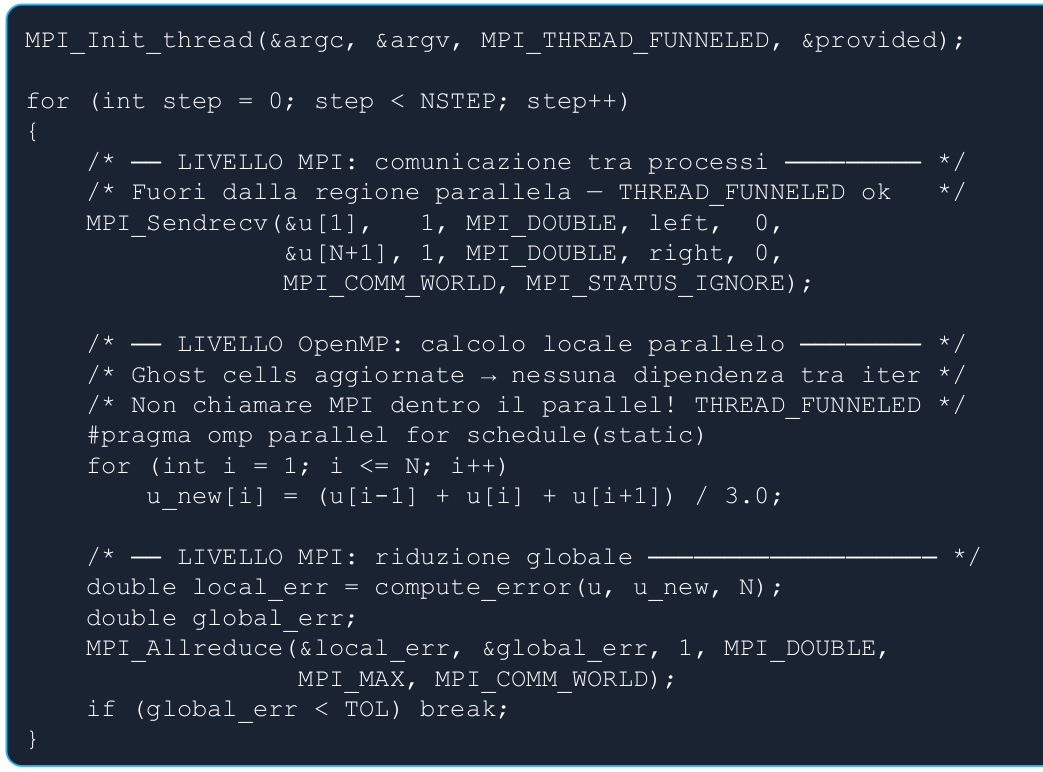
\includegraphics[width=0.8\linewidth]{Images/cap_9/esempio_codice_for.png}
\end{figure}
\subsubsection*{Analisi del pattern}
Il programma si struttura in un ciclo iterativo che alterna tre fasi distinte, coerenti con il livello di supporto \texttt{MPI\_THREAD\_FUNNELED}:
\begin{enumerate}
    \item \textbf{Fase di Comunicazione (Solo MPI):} Fuori dalla regione parallela, il master thread comunica con gli altri processi (es. scambio delle \textit{ghost cells} tramite \texttt{MPI\_Sendrecv}).
    \item \textbf{Fase di Calcolo (Solo OpenMP):} Viene aperta la regione parallela (\texttt{\#pragma omp parallel}). I thread eseguono il calcolo intensivo sui dati locali. All'interno di questa regione è \textit{severamente vietato} effettuare chiamate MPI.
    \item \textbf{Fase di Sincronizzazione (Solo MPI):} Chiusa la regione parallela, il master thread torna a essere l'unico operante e gestisce eventuali riduzioni globali (es. calcolo dell'errore massimo tramite \texttt{MPI\_Allreduce}) per decidere le sorti dell'iterazione.
\end{enumerate}
\section{Binding e Affinità nell'approccio ibrido}
Un programma ibrido MPI+OpenMP raggiunge prestazioni ottimali solo se i thread OpenMP sono esplicitamente legati (pinning/binding) ai core del nodo di elaborazione appartenenti al loro processo MPI. Questo evita la migrazione dei thread da parte del sistema operativo, ottimizzando l'uso della cache e minimizzando le penalità dell'architettura NUMA.

\subsection*{1. Configurazione dell'ambiente (OpenMP)}
Le variabili di ambiente istruiscono la libreria OpenMP su come gestire i thread prima dell'esecuzione:
\begin{verbatim}
export OMP_NUM_THREADS=4    # Numero di thread per processo MPI
export OMP_PROC_BIND=close  # Mantiene i thread vicini tra loro (stesso socket)
export OMP_PLACES=cores     # Assegna un thread per ogni core fisico
\end{verbatim}

\subsection*{2. Lancio dell'applicazione (MPI)}
In fase di lancio, è necessario mappare correttamente i processi e i thread sull'hardware tramite \texttt{mpirun}:
\begin{verbatim}
mpirun -np 2 \
  --bind-to socket \        # Assegna 1 processo MPI per ogni socket
  --map-by socket:pe=4 \    # Alloca 4 Processing Elements (thread) per processo
  ./programma_ibrido
\end{verbatim}

\subsection*{3. Verifica a runtime}
È buona norma verificare che l'assegnazione sia andata a buon fine. In Linux, si può utilizzare la funzione \texttt{sched\_getcpu()} all'interno di una regione parallela per stampare l'ID del core fisico su cui il thread è in esecuzione:
\begin{verbatim}
#pragma omp parallel
{
    printf("proc %d thread %d core %d\n",
           rank, omp_get_thread_num(), sched_getcpu());
}
\end{verbatim}

Nei nodi moderni (es. 2 socket per nodo), i dati vengono allocati vicino ai core che li generano/utilizzano per primi. Gli accessi alla memoria inter-socket (cross-socket) possono essere da 2 a 3 volte più lenti. L'utilizzo di \texttt{OMP\_PROC\_BIND=close} garantisce che sia i thread che i relativi dati risiedano sullo stesso socket hardware, abbattendo drasticamente i tempi di latenza.

\section*{Quando conviene il modello ibrido?}

Il modello ibrido MPI+OpenMP non rappresenta una soluzione universale. La sua efficacia dipende fortemente dalla struttura matematica del problema da risolvere e dalla frequenza delle comunicazioni in rete.

\subsection*{Quando CONVIENE l'approccio ibrido}
\begin{itemize}
    \item \textbf{Comunicazioni frequenti tra processi vicini:} In problemi con domini spaziali (es. calcolo tramite stencil, Equazioni Differenziali alle Derivate Parziali - PDE, simulazioni su griglia), la comunicazione è alta. Ridurre i processi MPI a favore dei thread riduce lo scambio dei bordi (\textit{halo exchange}) ad ogni iterazione.
    \item \textbf{Nodi hardware con molti core (32-128):} Lanciare 128 processi MPI sullo stesso nodo genera un overhead di sistema altissimo e uno spreco di memoria. Un singolo processo MPI con 128 thread OpenMP sfrutta in modo nettamente migliore la memoria condivisa.
\end{itemize}

\subsection*{Quando NON CONVIENE (Meglio MPI puro)}
\begin{itemize}
    \item \textbf{Problemi "imbarazzantemente paralleli":} Se i task sono indipendenti e la necessità di comunicazione è quasi nulla, un approccio puro MPI è più semplice da scrivere ed ugualmente efficiente.
    \item \textbf{Scarsa scalabilità locale di OpenMP:} Se il vostro codice parallelo locale non scala oltre gli 8-16 thread (es. a causa di colli di bottiglia fisici o logici), forzarlo è controproducente. In un nodo da 32 core, è preferibile una configurazione mista leggera (es. 4 processi MPI $\times$ 8 thread OpenMP) rispetto a una massiva (1 processo MPI $\times$ 32 thread).
    \item \textbf{Mancanza di tempo per lo sviluppo:} La programmazione ibrida aggiunge complessità a livello di scrittura, gestione della memoria e debugging. Il consiglio è iniziare con un approccio MPI puro e ottimizzarlo introducendo OpenMP solo successivamente, se necessario.
\end{itemize}

\vspace{0.5cm}
\begin{quote}
    \textbf{Regola pratica (Rule of Thumb):}
    Misurare sempre le prestazioni prima di alterare il codice (utilizzando tool come \texttt{perf} o le misurazioni con \texttt{MPI\_Wtime()}). Se il programma spende \textbf{più del 30\% del suo tempo totale di esecuzione all'interno di chiamate MPI}, l'approccio ibrido potrebbe offrire dei reali vantaggi.
\end{quote}

\section*{Compilazione, Linkaggio ed Esecuzione}

La gestione di un programma ibrido richiede accorgimenti specifici in fase di build e di esecuzione, poiché unisce i requisiti di due paradigmi differenti.

\subsection*{Build del progetto}
\begin{itemize}
    \item \textbf{Compilazione:} Si utilizza lo script/wrapper del compilatore MPI (es. \texttt{mpicc} o \texttt{mpicxx}) fornendogli esplicitamente il flag per abilitare OpenMP (ad esempio, \texttt{-fopenmp} per GCC).
    \item \textbf{Linkaggio:} Solitamente è gestito in automatico dal wrapper MPI. In alcuni ambienti potrebbe essere necessario specificare il linkaggio alla versione \textit{thread-safe} della libreria MPI.
\end{itemize}

\subsection*{Fase di Esecuzione}
I comandi di avvio (es. \texttt{mpirun}, \texttt{srun}) e la mappatura dell'hardware sono \textbf{altamente non portabili} e dipendono dal gestore di risorse del cluster (es. Slurm, PBS). Regole d'oro:
\begin{itemize}
    \item Assicurarsi di lanciare meno processi MPI rispetto al numero totale di core fisici disponibili sul nodo.
    \item Garantire che variabili d'ambiente cruciali (es. \texttt{OMP\_NUM\_THREADS}) vengano propagate correttamente a tutti i processi MPI allocati in rete, ad esempio passandole direttamente nella riga di comando dell'eseguibile (\texttt{env VAR=VALUE ./binario}).
\end{itemize}

\section*{Compilare da un singolo sorgente (Preprocessore C)}

Per evitare di mantenere versioni multiple dello stesso programma (seriale, puro MPI, puro OpenMP, ibrido), è prassi utilizzare le direttive del preprocessore C/C++ per isolare il codice parallelo.

\subsection*{Uso dei simboli predefiniti}
\begin{itemize}
    \item \texttt{\_OPENMP}: È una macro definita automaticamente dal compilatore quando viene passato il flag di attivazione di OpenMP.
    \item \texttt{USE\_MPI}: È una macro definita dall'utente a tempo di compilazione (tramite il flag \texttt{-DUSE\_MPI}) per includere le funzioni MPI.
\end{itemize}

\subsection*{Esempio di robustezza del codice}
Impostare i valori di default per \texttt{rank} e \texttt{size} garantisce che il programma possa funzionare correttamente anche se compilato in modalità puramente seriale (o solo OpenMP):

\begin{verbatim}
#ifdef _OPENMP
    // Codice e direttive OpenMP (attivo se flag -fopenmp presente)
#endif

/* Valori di fallback per l'esecuzione seriale */
int rank = 0;
int size = 1;

#ifdef USE_MPI
    // Codice MPI (attivo se flag -DUSE_MPI presente)
    MPI_Init(...);
    MPI_Comm_rank(MPI_COMM_WORLD, &rank);
    MPI_Comm_size(MPI_COMM_WORLD, &size);
#endif
\end{verbatim}

\section*{I diversi approcci alla programmazione parallela}

Esistono tre strategie principali per mappare un'applicazione parallela sulle moderne architetture HPC, che variano in base al bilanciamento tra memoria distribuita (MPI) e condivisa (OpenMP).

\begin{enumerate}
    \item \textbf{MPI puro:} 
    \begin{itemize}
        \item Viene lanciato 1 processo MPI per ogni singolo core fisico.
        \item Nessun utilizzo del threading.
        \item Massimo volume di comunicazione sulla rete.
    \end{itemize}
    
    \item \textbf{Completamente ibrido (Fully Hybrid):} 
    \begin{itemize}
        \item Viene lanciato 1 solo processo MPI per ogni nodo fisico.
        \item OpenMP gestisce la parallelizzazione \textit{intra-nodo} creando un thread per ogni core disponibile sul nodo.
        \item Minimizza il numero di processi MPI e il traffico di rete.
    \end{itemize}
    
    \item \textbf{Modalità mista (Mixed Mode):} 
    \begin{itemize}
        \item Rappresenta un compromesso: si lanciano più processi MPI per nodo (ad esempio uno per socket NUMA).
        \item Ogni processo MPI genera a sua volta un gruppo di thread OpenMP (es. un thread per core all'interno di quel socket).
        \item Spesso rappresenta il punto di massima efficienza (\textit{sweet spot}).
    \end{itemize}
\end{enumerate}

\section*{Associazione di thread e processi (Esempio pratico)}

La sintassi per allocare risorse ("pinning" o "binding") è altamente non portabile e dipende dalla toolchain utilizzata. 

\subsection*{Caso di studio: Mappatura Completamente Ibrida}
\textbf{Hardware target:} Un cluster composto da nodi \textit{dual-socket} (2 CPU per nodo), in cui ogni CPU possiede 6 core. Totale: 12 core per nodo.

\vspace{0.3cm}
Esempio di avvio utilizzando la toolchain \textbf{Intel MPI + Intel Compiler}:
\begin{verbatim}
OMP_NUM_THREADS=12 mpirun -ppn 1 -np 2 \
    -env KMP_AFFINITY scatter \
    ./a.out
\end{verbatim}

\textbf{Analisi dei parametri:}
\begin{itemize}
    \item \texttt{OMP\_NUM\_THREADS=12}: Genera 12 thread OpenMP per processo (occupando tutti i core del nodo).
    \item \texttt{-ppn 1}: (\textit{Processes Per Node}) Alloca esattamente 1 processo MPI su ciascun nodo fisico.
    \item \texttt{-np 2}: (\textit{Number of Processes}) Richiede 2 processi MPI in totale (impegnando così 2 nodi interi del cluster).
    \item \texttt{KMP\_AFFINITY scatter}: Variabile d'ambiente proprietaria Intel per il pinning. Distribuisce ("sparge") i thread in modo uniforme sui core fisici per evitare accavallamenti e massimizzare la banda di memoria.
\end{itemize}

\section*{MPI Puro: Pro e Contro}

Nonostante l'avvento dei sistemi multicore, l'approccio basato puramente su MPI (un processo per core, nessun thread) rimane una scelta valida e molto diffusa. Di seguito un'analisi dei vantaggi e degli svantaggi di questo modello.

\subsection*{Vantaggi (Pro)}
\begin{itemize}
    \item \textbf{Programmazione più semplice:} L'assenza di multithreading elimina completamente i problemi di sicurezza (\textit{thread safety}), evitando \textit{race conditions} e la necessità di meccanismi di mutua esclusione (\textit{lock}, semafori).
    \item \textbf{Gestione trasparente dell'hardware:} L'affinità dei processi e il posizionamento delle pagine di memoria (architettura ccNUMA) non sono un problema. Poiché la memoria è strettamente privata, i dati vengono allocati naturalmente sul nodo NUMA locale al processo chiamante.
    \item \textbf{Sfruttamento della rete:} Un elevato numero di processi può essere necessario e utile per saturare completamente la larghezza di banda dell'interconnessione di rete.
    \item \textbf{Analisi prestazionale lineare:} È presente un solo livello di overhead (la latenza di rete) e la scalabilità risponde a un solo livello della Legge di Amdahl, semplificando il profiling del codice.
\end{itemize}

\subsection*{Svantaggi (Contro)}
\begin{itemize}
    \item \textbf{Spreco di memoria (Dati replicati):} In un modello a memoria puramente distribuita, i dati globali necessari a tutti i \textit{worker} devono essere replicati nella memoria privata di ogni singolo processo. Su nodi con decine di core, questo porta a un rapido esaurimento della RAM.
    \item \textbf{Overhead di comunicazione:} Un numero massiccio di processi (es. 128 per nodo) genera un volume elevatissimo di messaggi, frammentando il traffico e causando potenziale congestione di rete.
    \item \textbf{Difficoltà nel bilanciamento del carico:} A differenza del threading (in cui il carico può essere redistribuito dinamicamente a costo quasi zero sulla memoria condivisa), in MPI il ribilanciamento richiede il trasferimento fisico dei dati attraverso la rete.
    \item \textbf{Mancanza di sovrapposizione garantita:} Risulta complesso strutturare il codice in modo da sovrapporre in modo efficiente le fasi di comunicazione con quelle di calcolo (una tecnica più semplice nel modello ibrido delegando la rete a un singolo thread dedicato).
    \item \textbf{Limiti architetturali:} Rende difficile sfruttare appieno i molteplici livelli di parallelismo offerti dall'hardware moderno.
\end{itemize}

\section*{Approccio Generale Multilivello}

Per sviluppare un'applicazione ibrida efficiente, è consigliabile adottare una strategia gerarchica in due fasi, partendo dal livello macroscopico fino ad arrivare a quello microscopico.

\subsection*{1. Parallelizzazione principale con MPI}
Il primo passo consiste nel decomporre il dominio globale del problema distribuendolo ai vari processi MPI. Esempi di decomposizione dei task includono:
\begin{itemize}
    \item Distribuzione delle frequenze (nei solver per equazioni delle onde).
    \item Decomposizione del dominio spaziale/griglia (nei solver ODE/PDE).
    \item Distribuzione dei gruppi di atomi (nelle simulazioni di dinamica molecolare).
\end{itemize}

\subsection*{2. Sfruttamento del parallelismo interno con OpenMP}
Una volta distribuiti i macro-task, si ottimizza l'elaborazione locale (intra-nodo):
\begin{itemize}
    \item Si utilizza un \textit{profiler} per individuare le sezioni di codice computazionalmente più intensive (gli \textit{hotspot}).
    \item Si applica OpenMP ai cicli interni più pesanti (es. ciclo sulle frequenze, calcolo locale delle forze interatomiche, aggiornamento degli elementi della mesh).
    \item Si misura sistematicamente l'efficienza per determinare il numero ottimale di thread da allocare per processo.
\end{itemize}


\section*{Cose su cui fare attenzione (Pitfalls)}

L'adozione del modello ibrido richiede cautela per non incorrere in degradi prestazionali.

\subsection*{L'utilità dei thread non è universale}
Non tutti i programmi MPI traggono reale beneficio dall'aggiunta di OpenMP:
\begin{itemize}
    \item In codici con parallelismo a grana grossa (\textit{loosely parallel}), dove le comunicazioni di rete sono già minime, l'ibrido è superfluo.
    \item L'overhead associato alla creazione e distruzione dei thread è stimabile nell'ordine di $10^4$ operazioni in virgola mobile (flops). Se il carico computazionale del ciclo è inferiore a questa soglia, OpenMP rallenterà l'esecuzione.
    \item È imperativo misurare empiricamente i tempi di esecuzione variando il rapporto processi/thread per trovare il \textit{bestseller point}.
\end{itemize}

\subsection*{Comunicazione MPI all'interno di regioni OpenMP}
Incrociare le comunicazioni di rete con le regioni parallele è rischioso:
\begin{itemize}
    \item L'architettura software diventa estremamente complessa se si permette a ogni singolo thread di effettuare operazioni MPI in modo indipendente.
    \item Molte implementazioni reali della libreria MPI presentano tuttora limitazioni tecniche o severi problemi di efficienza quando operano al massimo livello di supporto (\texttt{MPI\_THREAD\_MULTIPLE}), rendendo le comunicazioni concorrenti lente o instabili.
\end{itemize}